\documentclass[conference]{IEEEtran}
% \documentclass[journal,onecolumn]{IEEEtran}
\IEEEoverridecommandlockouts
% The preceding line is only needed to identify funding in the first footnote. If that is unneeded, please comment it out.
\usepackage{cite}
\usepackage{amsmath,amssymb,amsfonts}
\usepackage{algorithmic}
\usepackage{graphicx}
\usepackage[colorlinks=true, allcolors=blue]{hyperref}
\usepackage{url}
\usepackage{textcomp}
\usepackage{minted}
\usepackage{svg}
\usepackage{tabularx} % Allows creating tables with specified column widths
\usepackage{booktabs}
\usepackage{xcolor}
\usepackage[table]{xcolor}
\usepackage{colortbl}
\usepackage{multirow}
\usepackage{array}
\newcolumntype{C}[1]{>{\centering\arraybackslash}p{#1}}
\usepackage{adjustbox}
\usepackage{float}
\newminted{python}{
    linenos,
    autogobble,
    breaklines,
    fontsize=\scriptsize,
    frame=lines,
    framesep=2mm,
    bgcolor=black!5,
    rulecolor=\color{gray},
    framesep=3mm,
    baselinestretch=1.2,
    tabsize=4,
}
\usepackage[font=small,skip=0pt]{caption}
\captionsetup{skip=-0.001pt}
\usepackage{subcaption}
\captionsetup[subfigure]{aboveskip=-0.3pt}
\def\BibTeX{{\rm B\kern-.05em{\sc i\kern-.025em b}\kern-.08em
    T\kern-.1667em\lower.7ex\hbox{E}\kern-.125emX}}

\begin{document}

\title{Comparative Analysis of Neural Network-Based Techniques for Vehicular Location Prediction}
%Proactive Vehicular Location Prediction for 5G Radio Resource Allocation Using Neural Network-Based Techniques}

\author{\IEEEauthorblockN{Sina Ebrahimi}
\IEEEauthorblockA{\textit{Centre for Future Transport and Cities} \\
\textit{Coventry University}\\
Coventry, UK \\
ebrahimis@coventry.ac.uk}
}

\maketitle

\begin{abstract}
Vehicular location prediction is crucial for improving Quality of Service (QoS) in fifth-generation (5G) radio Resource Allocation (RA). This study presents a novel comparison of five Neural Network (NN) models—Recurrent NN (RNN), Long Short-Term Memory (LSTM), Gated Recurrent Unit (GRU), one-dimensional convolutional NN (Conv1D), and Multi-Layer Perceptron (MLP)—in predicting vehicle positions using a dataset of vehicular mobility traces from Seoul, South Korea. The models are assessed using metrics such as coefficient of determination ($\text{R}^2$ score), Root Mean Square Error (RMSE), loss over epochs, and execution time per epoch. Out of the models tested, the MLP model showed the best performance, with an RMSE of 0.42 meters and an $\text{R}^2$ score of 0.999992. This represents a 32\% decrease in RMSE compared to Conv1D and the recurrent models and a significantly higher $\text{R}^2$ score. Moreover, MLP demonstrated the most rapid convergence and the shortest average execution time per epoch, emphasizing its efficiency. The results suggest that using simpler architectures, such as MLP, is quicker and more effective for this particular task. This provides valuable information for designing proactive RA strategies in 5G networks.
\end{abstract}

\begin{IEEEkeywords}
Prediction, Vehicular Mobility, Proactive Mobility Prediction, 5G, Handover Management, Radio Resource Management, Neural Networks
\end{IEEEkeywords}

\section{Introduction} \label{introduction}
Fifth-generation (5G) wireless technology has enabled fast and responsive communication, which has greatly impacted sectors such as transportation. Especially in metropolitan areas, it is imperative to properly manage network resources for vehicle communications as vehicles are increasingly included in the Internet of Things (IoT) ecosystem. Radio Resource Management (RRM) is crucial in 5G networks as it optimizes network performance and guarantees Quality of Service (QoS) for users. Precise prediction of vehicle location can greatly improve RRM by facilitating proactive Resource Allocation (RA), enabling networks to allocate users to the most optimal base stations in advance of handovers \cite{7931566}. This proactive approach is critical for properly controlling the always-shifting traffic patterns in urban areas because it can significantly reduce delays and improve connectivity.

Several Neural Network (NN) structures, including Recurrent NN (RNN), Long Short-Term Memory (LSTM), Gated Recurrent Unit (GRU), Convolutional NN (CNN), and Multi-Layer Perceptron (MLP), have demonstrated potential in forecasting intricate patterns \cite{6795963,9204396}. Nevertheless, it is necessary to conduct a thorough analysis and evaluation of these architectures specifically in relation to vehicular location prediction for 5G RRM. This study aims to fill this void by assessing the efficacy of these NN architectures using vehicular mobility data obtained from Seoul, South Korea \cite{dataset20kumbhar}. The models are assessed in terms of their computational efficiency, rate of convergence, and capacity to precisely forecast, offering insightful information on their appropriateness for real-time 5G applications. This work is distinctive in that it compares several NN architectures to enhance vehicle location predictions.

The next sections of this paper are organized as follows: Literature is briefly reviewed in Sec. \ref{related-work}. The problem and dataset are introduced in Sec. \ref{dataset}. The various NN-assisted methods utilized in this paper are succinctly introduced in Sec. \ref{methods}. Sec. \ref{results} presents the experimental results. Ultimately, discussion and future work are provided in Sec. \ref{discussions}.


\section{Related Work} \label{related-work}
The ability of vehicle location prediction to improve 5G radio performance has recently gained significant interest. While CNN-based models have also been shown to extract spatial features from this kind of data, LSTM networks have been shown to be successful in capturing temporal relationships in mobility data. {\cite{9349962,7870510}. Within the context of 5G, scientists have looked at how Machine Learning (ML) methods might enhance network performance. Deep reinforcement learning techniques have specifically shown promise in optimizing joint mobility prediction and resource management \cite{7725934,tvt23choi}.

ML algorithms have enhanced handover management in 5G networks, reducing service failures and thus greatly improving QoS \cite{7792669,PRIYANKA2023100389}. Recent research suggests that simpler models such as MLP and one-dimensional convolutional NN (Conv1D) can occasionally achieve better performance than more complex recurrent architectures, especially in tasks involving spatio-temporal prediction. \cite{cikm23zhang} has demonstrated that MLP networks are successful in forecasting handovers in ultra-dense 5G networks, effectively managing intricate urban settings with exceptional precision and efficiency. Furthermore, Conv1D networks have demonstrated their efficacy in capturing localized patterns in sequential data, thus reinforcing the possibility of employing simpler models for mobility prediction tasks \cite{7870510}.

These studies demonstrate the potential utility of NN-based techniques in determining the location of vehicles in 5G RRM. However, further investigation is required to comprehensively compare the various deep learning-based architectures. The objective of this study is to evaluate different architectures and identify the most suitable approach for proactive RA in 5G networks, thus addressing the existing gap in knowledge.


\section{Dataset} \label{dataset}
The \texttt{vehicular mobility trace at Seoul, South Korea} dataset is accessed from IEEE DataPort \cite{dataset20kumbhar}. The dataset is collected by simulating vehicles in urban environment using SUMO, which exports XML files as the raw output\footnote{Please refer to \cite{sumo24fcd} for the complete set of features.} \cite{sumo24fcd}. The trace location in Seoul, South Korea has an area spanning over 2.5 × 1.5 km where there are are more than 30 intersections. A number of simulated vehicles are moving in the road topology. The dataset is introduced in a study regarding vehicular reliable routing that aims to select the routes with the longest connectivity time to efficiently deliver communication messages \cite{lcomm21kumbhar}, where the authors introduced a heuristic to solve their problem. However, our goal is different, as we aim to predict the location of each vehicle in the next time step. We use the sparse scenario introduced in \cite{dataset20kumbhar} to conduct this experiment.

As part of the preprocessing stage, we initially transform the XML file \texttt{OpenStreetMap Trace for a Sparse Traffic.xml} into a CSV file. Then, we remove features \texttt{type, lane, slope, pos} as they do not influence vehicle mobility. In order to improve readability and performance, we also convert the data type of the features \texttt{id} and \texttt{time} to integer. The preprocessed features are displayed in Table \ref{tab:features}. With the exception of \texttt{id} and \texttt{time}, all other features have a data type of float. Moreover, Fig. \ref{fig:location} shows the coordinates of all vehicles across all the time steps in the environment. Overall, there are \textit{6 features and 1,483,385 records (comprising 3592 unique vehicles and 8220 time steps)}. 

Each time step might include some vehicles, and there is time dependency for the mobility of each individual vehicle throughout time steps. In order to predict the behavior of each vehicle, which is moving independently of the others, we generate sequences of length 5 for each vehicle by applying the \texttt{group by} method. Each sequence contains 4 features of x, y, angle, and speed for 5 consecutive time step for a unique vehicle followed by its location (x and y coordinates) at the fifth time step. We split the data with 80-20\% ratio between train and test datasets.

\begin{figure}
    \centering
    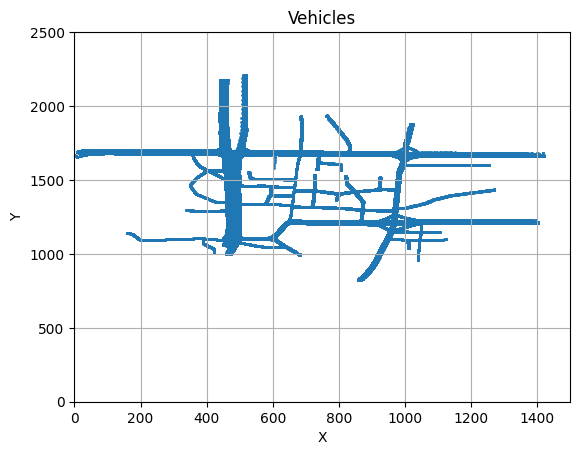
\includegraphics[width=0.7\linewidth]{figures/location.png}
    \caption{Location of all vehicles throughout all time steps \cite{dataset20kumbhar}}
    \label{fig:location}
\vspace{-2mm}
\end{figure}

\begin{table}
    \centering
    \scriptsize
    \caption{Dataset Features}
    \begin{tabular}{l|p{0.95cm}lp{4.6cm}}
        \textbf{Column}  &  Range & Unit & Description \cite{dataset20kumbhar} \\
        \hline
        \textbf{time} &  0 to 8219 & seconds & The time step described by the values within this timestep-element\\
        \textbf{id} & 0 to 4312 & - & The id of the vehicle\\
        \textcolor{blue}{\textbf{x}} & 2.14 to 1420.58 & meters & (longitude) The absolute X coordinate of the vehicle (center of front bumper). The value depends on the given geographic projection.\\
        \textcolor{blue}{\textbf{y}} & 820.68 to 2212.71 & meters & (latitude) The absolute Y coordinate of the vehicle (center of front bumper). \\
        \textbf{angle} & 0.0 to 360.0 & degrees & The angle of the vehicle in navigational standard (0-360 degrees, going clockwise with 0 at the 12'o clock position)\\
        \textbf{speed} & 0.0 to 37.38 & m/s & The speed of the vehicle\\
    \end{tabular}
    \label{tab:features}
    \captionsetup{singlelinecheck=false, justification=raggedright}
    \caption*{\centering \footnotesize *The blue features are the subject of prediction for individual vehicles.}
    \vspace{-5mm}
\end{table}

\section{Methods} \label{methods}
This section explains the fundamental models employed for predicting vehicle movement, focusing on RNN, LSTM, GRU, Conv1D, and MLP. Each model is chosen for its ability to capture temporal and spatial patterns in sequential data.

\begin{figure}
\vspace{-4mm}
    \centering
    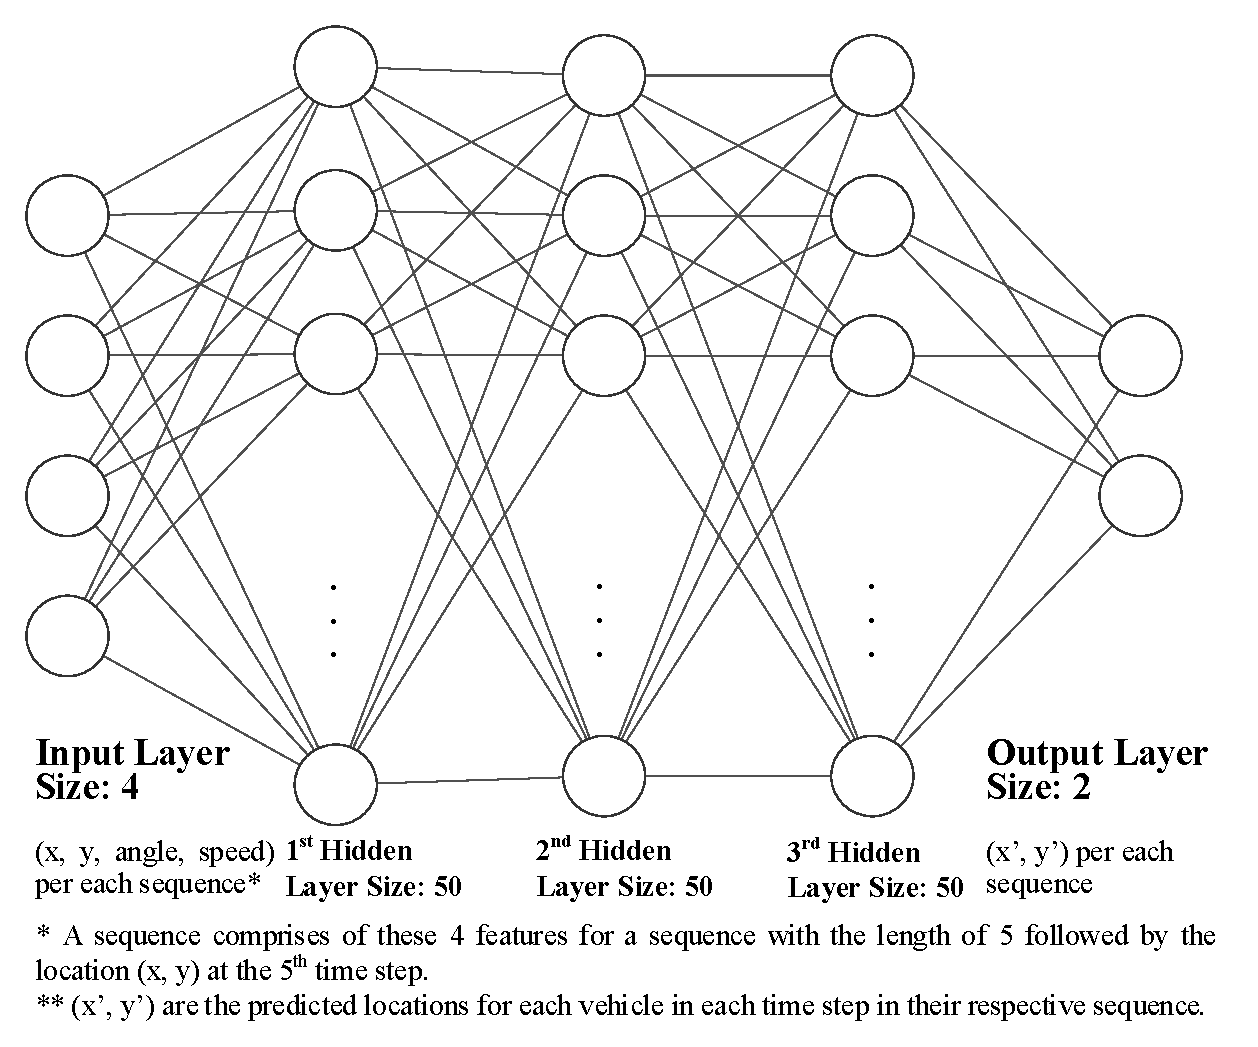
\includegraphics[width=1.06\linewidth]{figures/architecture.pdf}
    %\includesvg[width=\linewidth]{figures/architecture.svg}
    \caption{Generic NN architecture (Image generated using \cite{joss19lenail})}
    \label{fig:nn-architecture}
\vspace{-4mm}
\end{figure}

\subsection{RNN}
RNNs are designed for sequential data processing, utilizing a looped structure to retain information from previous time steps. This makes them suitable for tasks like time-series forecasting and vehicle movement prediction, where temporal data sequence is key. The RNN architecture consists of:
\begin{itemize}
    \item \textbf{Input Layer:} receives sequential data as input vectors at each time step.
    \item \textbf{Hidden Layers:} feature recurrent connections, allowing the network to preserve information over time. The hidden state \( h_t \) at time step \( t \) is calculated as:
    \[
    h_t = \sigma(W_{xh} \cdot x_t + W_{hh} \cdot h_{t-1} + b_h)
    \]
    where \( x_t \) is the input at \( t \), \( W_{xh} \) and \( W_{hh} \) are the weight matrices, \( b_h \) is the bias vector, and \( \sigma \) denotes the activation function (e.g., \texttt{tanh}).
    \item \textbf{Output Layer:} generates the output \( y_t \) for the current time step:
    \[
    y_t = \sigma(W_{hy} \cdot h_t + b_y)
    \]
    where \( W_{hy} \) represents the weight matrix that connects the hidden state to the output, and \( b_y \) is the bias vector.
\end{itemize}

RNNs are foundational for sequence modeling but can struggle with long-term dependencies due to vanishing gradients, making them better suited for short-term predictions \cite{prep23ghojogh}.

\subsection{LSTM}
LSTM networks extend RNNs by incorporating memory cells and gating mechanisms to handle long-term dependencies effectively \cite{6795963}. This makes them ideal for tasks requiring the retention of information over extended periods, like predicting vehicle trajectories based on historical data. The LSTM architecture includes:
\begin{itemize}
    \item \textbf{Input Layer:} sequential data enters the network at each time step.
    \item \textbf{LSTM Cells:} each cell contains forget (\( f_t \)), input (\( i_t \)), and output  (\( o_t \)) gates, which manage the flow of information:
    \[
    f_t = \sigma(W_f \cdot [h_{t-1}, x_t] + b_f), \quad i_t = \sigma(W_i \cdot [h_{t-1}, x_t] + b_i)
    \]
    \[
    \tilde{C}_t = \tanh(W_C \cdot [h_{t-1}, x_t] + b_C), \quad C_t = f_t \cdot C_{t-1} + i_t \cdot \tilde{C}_t
    \]
    \[
    o_t = \sigma(W_o \cdot [h_{t-1}, x_t] + b_o), \quad h_t = o_t \cdot \tanh(C_t)
    \]
    where \( C_t \) is the cell state.
    \item \textbf{Output Layer:} the final hidden state generates the prediction, which represents the next position of the vehicle.    
\end{itemize}

LSTMs are selected for their robustness in modeling complex temporal sequences, making them suitable for long-term vehicle trajectory prediction.

\subsection{GRU}
GRUs simplify the LSTM architecture by merging the input and forget gates into a single update gate, reducing complexity and computational cost while still capturing long-term dependencies \cite{prep23ghojogh}. The GRU architecture features:
\begin{itemize}
    \item \textbf{Input Layer:} sequential data is fed into GRU cells at each time step.
    \item \textbf{GRU Cells:} comprising reset (\( r_t \)) and update (\( z_t \)) gates that regulate information flow:
    \[
    r_t = \sigma(W_r \cdot [h_{t-1}, x_t] + b_r),  \quad z_t = \sigma(W_z \cdot [h_{t-1}, x_t] + b_z)
    \]
    \[
    \tilde{h}_t = \tanh(W_h \cdot [r_t \cdot h_{t-1}, x_t] + b_h),  h_t = z_t \cdot h_{t-1} + (1 - z_t) \cdot \tilde{h}_t
    \]
    where \( \tilde{h}_t \) represents the candidate activation, and \( h_t \) is the updated hidden state.
    \item \textbf{Output Layer:} generates the final prediction from \( h_t \).
\end{itemize}

GRUs are chosen for their efficiency and performance in tasks where both precision and computational resources are critical.

\subsection{Conv1D}
Conv1D models are used to analyze sequential data, utilizing convolutional filters to capture spatial hierarchies, making them effective for identifying local patterns in vehicle trajectory data \cite{jymssp21kiranyaz}. The Conv1D architecture includes:
\begin{itemize}
    \item \textbf{Input Layer:} the input data consists of sequences representing time-varying features, which are flattened before being fed into the input layer.
    \item \textbf{Convolutional Layers:} Conv1D layers utilize a collection of convolutional filters to process the input sequence. The filters move across the input, capturing specific characteristics in the surrounding area:
    \[
    z_t = \sum_{i=1}^{k} w_i \cdot x_{t+i-1} + b
    \]
    where \( k \) is the kernel size, \( w_i \) are the filter weights, and \( b \) is the bias term.
    \item \textbf{Pooling Layers:} reduce dimensionality, typically using max pooling to retain key features.
    \item \textbf{Fully Connected (Dense) Layer:} aggregates features to produce the final output.
\end{itemize}

Conv1D models excel at capturing local dependencies, providing an alternative to recurrent networks by emphasizing local feature extraction.

\subsection{MLP}
MLPs are feedforward NNs consisting of multiple layers of interconnected neurons, capable of learning complex, non-linear relationships between input features and output predictions \cite{cikm23zhang}. The MLP architecture comprises:
\begin{itemize}
    \item \textbf{Input Layer:} receives flattened sequential data.
    \item \textbf{Hidden Layers:} each layer \( l \) performs a weighted sum of inputs followed by a non-linear activation function (i.e. 
Rectified Linear Unit (\texttt{ReLU})):
    \[
    h^{(l)} = \sigma(W^{(l)} \cdot h^{(l-1)} + b^{(l)})
    \]
    where \( h^{(l)} \) is the output of the \( l \)-th layer, \( W^{(l)} \) is the weight matrix, and \( b^{(l)} \) is the bias vector.
    \item \textbf{Output Layer:} provides the predicted output.
\end{itemize}

Although MLPs do not explicitly incorporate temporal dependencies, they can be utilized for predicting vehicle movement by considering the sequential data as a collection of features. This allows for the learning of non-linear relationships between past movements and future positions. MLPs are employed as a reference model to evaluate the influence of integrating temporal structures in prediction tasks. They offer a direct method for modeling relationships within the data, acting as a benchmark for more intricate models such as RNNs, LSTMs, and Conv1D networks.

Fig. \ref{fig:nn-architecture} illustrates a generic architecture for all the methods, assuming the presence of three layers, each consisting of 50 neurons. The depicted diagram resembles MLPs and does not illustrate the complexities of other techniques (such as the forget gate in LSTM), despite the fact that all these methods have the same number of layers and neurons. For more detailed information about the models (e.g., utilized activation functions), please refer to step 3 in Sec. \ref{tuning-annex}.

%%%%%%%%%%%%%%%%%%%%
\section{Experimental Results} \label{results}
The experiments were performed using PyTorch and widely used Python libraries on an NVIDIA Tesla K80 GPU. This section provides an overview of the metrics used to compare models, the process of tuning hyperparameters, and the comparative analysis of five NN-based techniques using the selected hyperparameters. The Adam optimizer was consistently employed in all methods to minimize the loss during training \cite{KingBa15}, with Mean Square Error (MSE) serving as the loss function in all experiments.

Different activation functions and techniques were utilized in each of the five NN architectures to improve performance. The LSTM and GRU models employ the \texttt{tanh} activation function as the default choice for their recurrent units, and the final output is then processed through a linear layer. The RNN model also employs a \texttt{tanh} activation function in the recurrent layer, which is then followed by a linear layer. The Conv1D model utilizes the \texttt{ReLU} activation function after each convolutional layer, followed by max pooling. The model then concludes with global average pooling before reaching a fully connected layer. The MLP model employs the \texttt{ReLU} activation function following each linear layer. Additionally, the input data is flattened to ensure compatibility with the fully connected structure of the network.

\subsection{Metrics}
The efficacy of the location prediction models was assessed using fundamental metrics: Root Mean Square Error (RMSE), Mean Absolute Error (MAE), and the coefficient of determination ($\text{R}^2$ score). In addition, we monitored the loss function throughout the epochs and documented the average time it took to complete each epoch.

\paragraph{RMSE}
is a metric that measures the magnitude of the differences between predicted and actual values. It emphasizes larger errors by squaring the discrepancies. Smaller RMSE values indicate higher model accuracy \cite{cr05willmott}. The study emphasizes the significance of RMSE as it offers a quantitative assessment of the overall precision of the models' predictions. Smaller RMSE values indicate better performance of the models.

\paragraph{MAE}
is a metric that calculates the average of the absolute differences between predicted and actual values. It provides a straightforward measure of prediction error without giving more importance to larger errors. It provides additional information to RMSE by giving a better understanding of the accuracy of predictions, especially in terms of the typical sizes of errors \cite{cr05willmott}.

\paragraph{$\text{R}^2$ Score}
quantifies the amount of variability in the dependent variable that can be explained by the model. A higher value, with a maximum of 1, indicates a more robust correlation with the data. It is crucial to comprehend the model's ability to explain things effectively \cite{biomet91nagelkerke}.

\paragraph{Loss}
was monitored throughout all epochs to assess the convergence and stability of the model during training. Lower loss values suggest better model performance in fitting the training data \cite{mit16goodfellow}.

\paragraph{Average Execution Time per Epoch}
is important for assessing computational efficiency, helping balance accuracy with time constraints in practical applications \cite{jproc17sze}.

\subsection{Hyperparameter Tuning}
Optimizing NN model performance requires thorough hyperparameter tuning \cite{mit16goodfellow}. We analyzed different arrangements using a hyperparameter grid (Table \ref{tab:tuning-values}).

\begin{table}[h!]
\centering
\caption{Hyperparameter Grid for Tuning}
\label{tab:tuning-values}
\begin{tabular}{l|p{4cm}}
\textbf{Hyperparameter} & \textbf{Values} \\
\hline
Hidden Size & 50, 100 \\
No. of Layers & 2, 3, 4 \\
Learning Rate & 0.1, 0.05, 0.01, 0.005, 0.001, 0.0005, 0.0001, 0.00005 \\
No. of Epochs & 30 \\
\end{tabular}
\end{table}

The grid search resulted in 48 unique combinations of hyperparameters, enabling a thorough examination of the hyperparameter space to determine the most optimal configurations for each method. To expedite the process, we assessed every combination by utilizing 10\% of the training and test datasets. The RMSE, $\text{R}^2$ scores, average wall-clock time, and convergence of the loss value over episodes for each method were evaluated using the specified combinations, as described in Sec. \ref{tuning-annex}. The hyperparameter sets selected for final analysis are highlighted in green in Table \ref{tab:top-experiments-tuning}.

\setlength{\tabcolsep}{2pt}
\begin{table}[htbp]
\centering
\caption{Top Experiments for Each Method Using Different Hyperparameters.}
\label{tab:top-experiments-tuning}
\resizebox{\columnwidth}{!}{%
\begin{tabular}{p{0.12\columnwidth}p{0.09\columnwidth}p{0.1\columnwidth}p{0.1\columnwidth}p{0.1\columnwidth}p{0.1\columnwidth}p{0.14\columnwidth}p{0.15\columnwidth}p{0.12\columnwidth}p{0.08\columnwidth}}
\hline
\textbf{Method} & \textbf{Hidden Size} & \textbf{Layers} & \textbf{$\alpha$} & \textbf{RMSE} & \textbf{MAE} & \textbf{$\text{R}^2$ Score} & \textbf{Avg Epoch Time} & \textbf{Final Loss} & \textbf{Final Epoch} \\
\hline
\multirow{3}{*}{\textbf{RNN}} & \rowcolor{green!30} 100 & 2 & 5e-4 & 16.26 & 11.05 & 0.9890 & 18.12 & 115.46 & 30 \\
 & 100 & 2 & 1e-3 & 59.52 & 41.63 & 0.8712 & 18.25 & 3824.85 & 30 \\
 & 100 & 2 & 5e-2 & 180.51 & 126.69 & -0.0470 & 18.2 & 35930.73 & 5 \\ \hline
\multirow{3}{*}{\textbf{LSTM}} & \rowcolor{green!30} 100 & 4 & 5e-4 & 10.8 & 6.68 & 0.9959 & 23.69 & 53.01 & 30 \\
 & 100 & 2 & 5e-4 & 10.76 & 7.3 & 0.9956 & 20.525 & 67.74 & 30 \\
 & 100 & 2 & 1e-3 & 12.49 & 8.39 & 0.9947 & 20.39 & 213.96 & 30 \\ \hline
\multirow{3}{*}{\textbf{GRU}} & \rowcolor{green!30} 100 & 3 & 5e-4 & 10.68 & 6.84 & 0.9962 & 22.88 & 104.95 & 30 \\
 & 100 & 2 & 5e-4 & 14.43 & 10.81 & 0.9933 & 21.95 & 96.07 & 30 \\
 & 50 & 3 & 1e-3 & 16.68 & 10.71 & 0.9901 & 21.16 & 410.59 & 30\\ \hline
\multirow{3}{*}{\textbf{Conv1D}} & \rowcolor{green!30} 50 & 3 & 1e-4 & 0.62 & 0.37 & 0.999985 & 18.44 & 0.83 & 30 \\
 & 50 & 3 & 5e-4 & 0.525 & 0.4 & 0.999991 & 18.45 & 1.9 & 30 \\
 & 50 & 2 & 1e-4 & 0.78 & 0.5 & 0.999976 & 16.73 & 0.67 & 30 \\ \hline
\multirow{3}{*}{\textbf{MLP}} & \rowcolor{green!30} 100 & 3 & 5e-5 & 0.42 & 0.23 & 0.999992 & 15.78 & 0.36 & 30 \\
 & 50 & 2 & 1e-4 & 0.525 & 0.41 & 0.999990 & 14.3 & 0.35 & 30 \\
 & 100 & 2 & 1e-4 & 0.525 & 0.36 & 0.999988 & 14.41 & 0.38 & 30 \\
\hline
\end{tabular}}
\vspace{-4mm}
\end{table}

\subsection{Methods Comparison} \label{sec-comparison}
\begin{figure*}
    \centering
    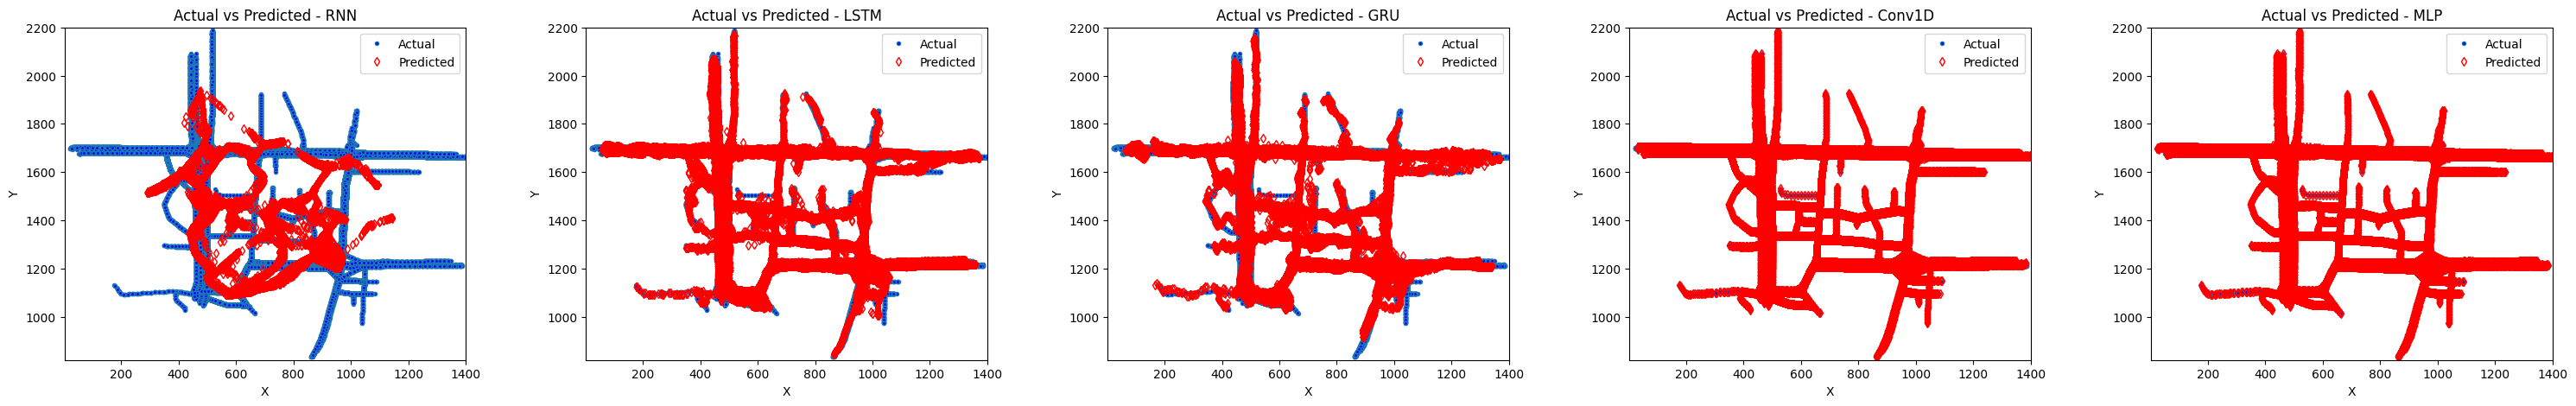
\includegraphics[width=\textwidth]{figures/all_vehicles_comparison.png}
    \caption{Visualization of predicted and actual locations for all vehicles across all time steps using five different methods.}
    \label{fig:pred-vs-actual-all-vehicles}
\end{figure*}

\begin{figure*}
    \centering
    \includesvg[width=\textwidth]{figures/vehicle_4225_comparison.svg}
    \caption{Visualization of predicted and actual locations for a random vehicle across all time steps using five different methods (1).}
    \label{fig:pred-vs-actual-random-vehicle-1}
\end{figure*}

\begin{figure*}
    \centering
    \includesvg[width=\textwidth]{figures/vehicle_3726_comparison.svg}
    \caption{Visualization of predicted and actual locations for a random vehicle across all time steps using five different methods (2).}
    \label{fig:pred-vs-actual-random-vehicle-2}
\end{figure*}

Several NN architectures—RNN, LSTM, GRU, Conv1D, and MLP—are compared in this part. Using the previously mentioned metrics helps one evaluate the performance. The further study is based on the ideal hyperparameter configuration for every method, shown by the green highlighting in Table \ref{tab:top-experiments-tuning}. It is crucial to mention that when predicting vehicle positions (x and y coordinates), the units for RMSE, MAE, and loss (calculated using MSE) are expressed in meters (m).

\paragraph{Visualizing predicted locations}
Fig. \ref{fig:pred-vs-actual-all-vehicles} displays the projected and real positions of all vehicles throughout all time intervals for all the utilized techniques. The predictions made by MLP and Conv1D closely align with the actual locations, whereas RNN fails to accurately detect vehicle locations. Nevertheless, the graph is excessively congested to analyze. Hence, in Figs. \ref{fig:pred-vs-actual-random-vehicle-1} and \ref{fig:pred-vs-actual-random-vehicle-2}, we examine the paths of two random vehicles over a period of time for a more detailed analysis. The forecasting performed by Conv1D and MLP techniques is exceptional. Nevertheless, the LSTM and GRU methods fail to accurately predict the locations of some of the sampled vehicles. Furthermore, the RNN method exhibits significant disparities between actual and predicted locations.

\paragraph{RMSE, MAE, and $\text{R}^2$ Score Comparison}
As depicted in Fig. \ref{fig:rmse-mae-r2-methods}, the MLP model surpasses all other methods in terms of the important metrics. The achieved RMSE is 0.42 meters, which is roughly 32\% lower than the RMSE of the second-best Conv1D model, which is 0.62 meters. In addition, the MLP model achieves an MAE of 0.23 meters, which is 38\% superior to the Conv1D model's MAE of 0.37 meters. The coefficient of determination ($\text{R}^2$) score for the MLP model is likewise the highest, reaching 0.999992. This value suggests an almost flawless level of prediction accuracy. This demonstrates the exceptional aptitude of MLP in precisely predicting vehicle positions with remarkable accuracy and a minimal error margin.

Although MLP outperforms Conv1D, Conv1D still shows strong performance with an RMSE of 0.62 meters and an MAE of 0.37 meters. On the other hand, the conventional recurrent models (RNN, LSTM, and GRU) demonstrate considerably higher RMSE and MAE values, with RNN doing the poorest. For example, the RMSE of the RNN is 16.26 meters, which is almost 38.7 times greater than the RMSE of the MLP. The notable disparity underscores the constraints of basic recurrent architectures in comprehending the intricate dynamics of vehicle movements compared to more straightforward models such as MLP and Conv1D.

\begin{figure}
    \centering
    \includesvg[width=1.09\linewidth]{figures/rmse-mae-r2score-methods.svg}
    \caption{RMSE, MAE, and $\text{R}^2$ score of the final epoch for various methods.}
    \label{fig:rmse-mae-r2-methods}
    \vspace{-4mm}
\end{figure}

\paragraph{Loss Over Epochs}
Convergence pertains to the speed and efficiency at which the loss function of each model reaches a stable minimum value during the training phase. As seen in Fig. \ref{fig:loss-over-epochs}, the MLP method shows the fastest and most constant convergence. Its loss from 6248.56 in the first epoch to roughly 0.11 by the 27th epoch clearly shows effective learning with almost no oscillations. Although the Conv1D approach has a slower pace, it exhibits satisfactory convergence, reaching a loss of around 3.45 by the 11th epoch and maintaining stability. These findings indicate that simpler models like MLP and Conv1D may optimize their weights more efficiently, rendering them highly effective for this particular task.

On the other hand, LSTM and GRU exhibit slower and less consistent convergence, reaching final losses of 22.59 and 174.87, respectively, by the 30th epoch. The GRU approach required only 12 epochs to complete and did not require further progression. The RNN model demonstrates the most significant challenge, as evidenced by its highest ultimate loss of 174.87. This indicates difficulties in accurately identifying the fundamental patterns within the data. The RNN model attained its minimum recorded loss of 116.77 meters in the 10th epoch. LSTM and GRU, despite their theoretical advantages for sequential data, necessitate a greater number of epochs for complete optimization and display more volatility during training due to their intricate structures. This investigation demonstrates that MLP and Conv1D not only produce lower loss values, but they also do it more effectively, rendering them more appropriate for this particular location prediction task.

\begin{figure}
        \centering
        \includesvg[width=0.71\linewidth]{figures/loss-over-epochs.svg}
        \caption{Loss (based on MSE) per epoch for different methods.}
        \label{fig:loss-over-epochs}
        \vspace{-4mm}
\end{figure}

\paragraph{Execution Time Per Epoch}
With the Conv1D model closely behind, Fig. \ref{fig:exec-time-over-epochs} shows that the MLP model displays the lowest average execution time per epoch. MLP's simplicity—that which includes fully connected layers free from sequential processing—helps to explain its computational efficiency. More effective than other methods is Conv1D, which employs convolutional operations. This results from the slower stride used for pooling layers, which guarantees accuracy while accelerating data processing.

On the other hand, recurrent models, specifically LSTM and GRU, have longer execution times per epoch. The LSTM model, for instance, has an average epoch duration of 23.69 seconds, which is over 50\% longer than the MLP model's 15.78 seconds. The longer execution time is due to the complexity of the LSTM and GRU architectures. They have to process sequential data and keep hidden states between time steps, which makes them harder to compute.

\begin{figure}
        \centering
        \includesvg[width=0.84\linewidth]{figures/exec-time-per-epoch.svg}
        \caption{Wall-clock time per epoch for different methods.}
        \label{fig:exec-time-over-epochs}
        \vspace{-4mm}
\end{figure}

\section{Conclusion} \label{discussions}
% (5 marks) Should present the summary of the findings (1-2 pages). Also provide what future work can be conducted on this project.
MLP emerged as the best-performing model in all categories, combining high prediction accuracy with excellent computational efficiency. Conv1D also demonstrated strong and consistent performance, making it a viable choice. While RNN, LSTM, and GRU are theoretically advantageous for sequence modeling, they are less suitable for accurate and efficient vehicle location prediction in this context.

The differences in architecture between these models are most likely to explain the findings. The MLP's fully connected layers are ideal for the small input size and specific nature of this prediction task, allowing it to reach high precision quickly. Conv1D's convolutional layers accurately capture spatial relationships, yielding high precision and short wall-clock times. On the other hand, the iterative nature of RNN, LSTM, and GRU, though beneficial in some sequential tasks, adds unnecessary complexity for this particular forecasting application. 

Our study indicates that MLP and Conv1D models outperform traditional recurrent models (RNN, LSTM, GRU) in vehicular location prediction for 5G RRM. The MLP model performed particularly well on metrics such as $\text{R}^2$ score, RMSE, MAE, and computational efficiency. These findings call into question the widespread belief that recurrent models are always superior for sequential data handling. Instead, they propose that simpler architectures like MLP and Conv1D might work better for some prediction tasks. These architectures offer faster training and inference times, which are important for real-time 5G applications, while still being able to capture patterns in space and time.

Future research should prioritize the integration of these models into a proactive 5G RRM framework. This integration should make use of their predictive capabilities to optimize network resources by taking into account the expected positions of vehicles. Furthermore, investigating hybrid models that integrate the advantages of MLP, Conv1D, and recurrent architectures could improve prediction accuracy in more intricate settings. Additional research should evaluate the ability of these models to be expanded and applied in larger and denser urban settings, as well as their effectiveness in different traffic situations. Evaluating the models' capacity to adapt to changing mobility patterns and resilience to different data sampling rates would give substantial insight for practical application. Incorporating effective location prediction into 5G RRM enables the development of intelligent, user-centric networks capable of consistently delivering QoS in extremely mobile environments.


\bibliographystyle{ieeetr} 
\bibliography{main}{}

\begin{appendices}
\section{Hyperparameter Tuning} \label{tuning-annex}
In this section, we define our models and hyperparameter grid to execute the experiments in order to choose the best hyperparameters for each method. In addition, one can find the code publicly on a \href{https://github.com/sinaebrahimi/Location_Prediction_-ANN-7088CEM-Project-}{Github repository}. In what follows, we rank sets of hyperparameters for each of the methods according to their RMSE, MAE, $\text{R}^2$ score, average epoch execution time, and loss slope (based on MSE) (also, see Tables \ref{tab:tuning-values} and \ref{tab:top-experiments-tuning}). Additionally, we will determine the optimal hyperparameter set for each method.

\paragraph{RNN}
Fig. \ref{fig:rmse-rnn} displays the RMSE metric for the RNN approach using various hyperparameters. The results indicate that selecting a learning rate ($\alpha$) of 0.0005 and employing 2 hidden layers, each containing 100 neurons, yields the minimum RMSE value. Furthermore, Fig. \ref{fig:r2-rnn} shows the coefficient of determination ($\text{R}^2$ score) for the RNN technique using various hyperparameters. The findings indicate that employing a RNN with two hidden layers and 100 neurons yields favorable outcomes when utilizing 0.0005 and 0.001 as $\alpha$. Hence, the hyperparameter set for the RNN method that is deemed optimal is $\alpha=0.0005$ with 2 hidden layers, each consisting of 100 neurons.

\begin{figure}[htbp]
    \centering
    \begin{subfigure}[b]{0.5\linewidth}
        \centering
        \includesvg[width=\textwidth]{figures/rmse-rnn.svg}
        \caption{}
        \label{fig:rmse-rnn}
    \end{subfigure}%
    \begin{subfigure}[b]{0.5\linewidth}
        \centering
        \includesvg[width=\textwidth]{figures/r2-rnn.svg}
        \caption{}
        \label{fig:r2-rnn}
    \end{subfigure}
    \caption{a) RMSE and b) $\text{R}^2$ score of the RNN method with different hyperparameters.}
    \label{fig:rnn-hypers}
    \vspace{-4mm}
\end{figure}

\paragraph{LSTM}
Fig. \ref{fig:rmse-lstm} illustrates the RMSE metric for the LSTM approach with different hyperparameters. The findings suggest that choosing 0.0005 and 0.001 as the values for $\alpha$ and utilizing either 2 hidden layers, each consisting of 100 neurons, results in the lowest RMSE value. Furthermore, Fig. \ref{fig:r2-lstm} displays the $\text{R}^2$ score of the LSTM technique using various hyperparameters. The findings indicate that using a LSTM model with two hidden layers and 100 neurons leads to favorable results when using 0.0005 as $\alpha$. Therefore, the most effective hyperparameter configurations for the LSTM technique includes two layers, with each layer comprising 100 neurons, and a $\alpha$ value of 0.0005.

\begin{figure}[htbp]
    \centering
    \begin{subfigure}[b]{0.5\linewidth}
        \centering
        \includesvg[width=\textwidth]{figures/rmse-lstm.svg}
        \caption{}
        \label{fig:rmse-lstm}
    \end{subfigure}%
    \begin{subfigure}[b]{0.5\linewidth}
        \centering
        \includesvg[width=\textwidth]{figures/r2-lstm.svg}
        \caption{}
        \label{fig:r2-lstm}
    \end{subfigure}
    \caption{a) RMSE and b) $\text{R}^2$ score of the LSTM method with different hyperparameters.}
    \label{fig:lstm-hypers}
    \vspace{-4mm}
\end{figure}

\paragraph{GRU}
Fig. \ref{fig:rmse-gru} displays the RMSE metric for the GRU method across different hyperparameters. The results suggest that selecting 0.0005 as the value of $\alpha$ and using 3 hidden layers, each comprising of 100 neurons, yields the minimum RMSE value. Moreover, Fig. \ref{fig:r2-gru} illustrates the $\text{R}^2$ score for the GRU technique with various hyperparameters. The results suggest that using a GRU with three hidden layers and 100 neurons produces acceptable results when $\alpha$ is set to 0.0005. Therefore, the hyperparameter configuration considered to be the best for the GRU method is $\alpha=0.0005$ with 3 hidden layers, each containing 100 neurons.

\begin{figure}[htbp]
    \centering
    \begin{subfigure}[b]{0.5\linewidth}
        \centering
        \includesvg[width=\textwidth]{figures/rmse-gru.svg}
        \caption{}
        \label{fig:rmse-gru}
    \end{subfigure}%
    \begin{subfigure}[b]{0.5\linewidth}
        \centering
        \includesvg[width=\textwidth]{figures/r2-gru.svg}
        \caption{}
        \label{fig:r2-gru}
    \end{subfigure}
    \caption{a) RMSE and b) $\text{R}^2$ score of the GRU method with different hyperparameters.}
    \label{fig:gru-hypers}
    \vspace{-4mm}
\end{figure}

\paragraph{Conv1D}
Fig. \ref{fig:rmse-conv1d} displays the RMSE metric for the Conv1D method, showcasing its performance across various hyperparameters. The findings indicate that selecting any combination of layers and neurons can yield positive outcomes within the range of $0.00005 \le \alpha \le 0.01$. However, despite the RMSE being fairly similar within this range, the smallest RMSE is observed when $\alpha$ is set to 0.0005, and there are three hidden layers, each consisting of 50 neurons. Furthermore, Fig. \ref{fig:r2-conv1d} illustrates the $\text{R}^2$ score for the Conv1D technique using different hyperparameters. These results also indicate the same conclusion as the RMSE metric, although the experiments (hidden size = 100, no. of layers = 3, $\alpha$ = 0.001), (hidden size = 50, no. of layers = 3, $\alpha$ = 0.01), (hidden size = 100, no. of layers = 2, $\alpha$ = 0.01), and (hidden size = 50, no. of layers = 4, $\alpha$ = 0.005) are nearly identical to the selected set using the RMSE metric. Therefore, we employ a method that utilizes three hidden layers, each consisting of 50 neurons, and a learning rate of $\alpha=0.0005$. 

\begin{figure}[htbp]
    \centering
    \begin{subfigure}[b]{0.5\linewidth}
        \centering
        \includesvg[width=\textwidth]{figures/rmse-conv1d.svg}
        \caption{}
        \label{fig:rmse-conv1d}
    \end{subfigure}%
    \begin{subfigure}[b]{0.5\linewidth}
        \centering
        \includesvg[width=\textwidth]{figures/r2-conv1d.svg}
        \caption{}
        \label{fig:r2-conv1d}
    \end{subfigure}
    \caption{a) RMSE and b) $\text{R}^2$ score of the Conv1D method with different hyperparameters.}
    \label{fig:conv1d-hypers}
    \vspace{-4mm}
\end{figure}

\paragraph{MLP}
Fig. \ref{fig:rmse-mlp} illustrates the RMSE metric for the MLP method across several hyperparameters. The findings indicate that favorable results can be attained by selecting any configuration of layers and neurons within the specified range of $0.00005 \le \alpha \le 0.01$. However, upon closer examination, it is evident that the optimal RMSE may be attained by utilizing only 2 layers, with each layer consisting of 50 neurons, when $\alpha$ is set to 0.001. Furthermore, Fig. \ref{fig:r2-mlp}  displays the $\text{R}^2$ score for the MLP technique with various hyperparameters. These results support the identical conclusion as the RMSE metric. Hence, a learning rate of 0.001, along with 2 hidden layers and 50 neurons, is considered acceptable. However, other configurations, such as those with learning rates of 0.00005 and 0.0001, regardless of their layer count and neuron size, are also very similar to the chosen hyperparameter set.

\begin{figure}[htbp]
    \centering
    \begin{subfigure}[b]{0.5\linewidth}
        \centering
        \includesvg[width=\textwidth]{figures/rmse-mlp.svg}
        \caption{}
        \label{fig:rmse-mlp}
    \end{subfigure}%
    \begin{subfigure}[b]{0.5\linewidth}
        \centering
        \includesvg[width=\textwidth]{figures/r2-mlp.svg}
        \caption{}
        \label{fig:r2-mlp}
    \end{subfigure}
    \caption{a) RMSE and b) $\text{R}^2$ score of the MLP method with different hyperparameters.}
    \label{fig:mlp-hypers}
    \vspace{-4mm}
\end{figure}
\end{appendices}

\end{document}
